% Use xelatex to generate a pdf file of this presentation.
%
% Standalone, style-matched companion to
%   ../left-join-pattern-bottlenecks/presentation.tex
% Two frames describing the ARCHITECTURE of the pg_log_query_plan()
% feature (commit "Add function to log the plan of the currently
% running query"):
%   1. the cross-backend request path and its triple deferral;
%   2. the "wrap, don't print" safe-point mechanism.
% The frames are self-contained -- lift either \begin{frame}..\end{frame}
% straight into another Copenhagen deck; the only dependencies are the
% pgblue/pgorange colours and the tikz libraries loaded below.

\documentclass{beamer}
\usepackage[english]{babel}
\usetheme{Copenhagen}

\usepackage{tikz}
\usetikzlibrary{positioning,calc,arrows.meta}

\setbeamertemplate{navigation symbols}{}

\definecolor{pgblue}{HTML}{336791}
\definecolor{pgorange}{HTML}{E8781A}

\title[pg\_log\_query\_plan]{Logging the plan of a running query}
\author{Andrei Lepikhov}
\institute{pgEdge}
\date{2026}

\begin{document}

% ---------------------------------------------------------------------
% SLIDE 1 -- the request path.
%
% Story: pg_log_query_plan() is a cross-backend request that is handled
% in THREE hops, each one deferring the real work to a point where more
% is safe to do:
%   1. signal handler   -- async-signal context: may only set a flag;
%   2. CHECK_FOR_INTERRUPTS -- may ereport, but the executor state at an
%      arbitrary interrupt point is unknown, so EXPLAIN is unsafe -->
%      it only re-arms the node wrappers (see slide 2);
%   3. node entry       -- executor is in a consistent state --> print.
%
% Left column = requester backend; the dashed box on the right = target
% backend, holding the vertical 3-hop pipeline.  The signal crosses the
% gap; the deferral condition rides each vertical arrow.
% ---------------------------------------------------------------------
\begin{frame}\frametitle{Architecture: from request to log line}
\vspace{-3mm}
\begin{center}
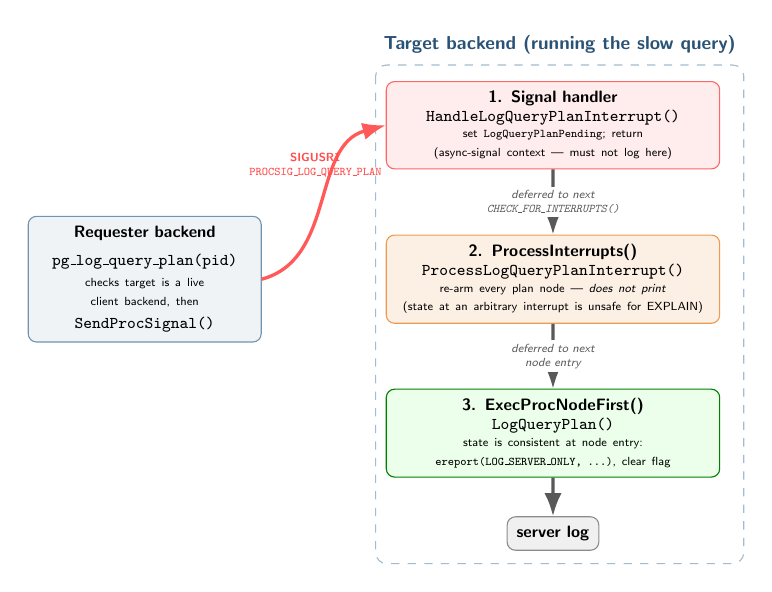
\begin{tikzpicture}[scale=0.85, every node/.append style={transform shape},
  proc/.style={draw=pgblue!70, rounded corners=3pt, fill=pgblue!8,
               align=center, font=\sffamily\scriptsize, inner sep=4pt,
               text width=3.2cm},
  handler/.style={draw=red!60, rounded corners=3pt, fill=red!7,
               align=center, font=\sffamily\scriptsize, inner sep=4pt,
               text width=4.7cm},
  cfi/.style={draw=pgorange!75, rounded corners=3pt, fill=pgorange!12,
               align=center, font=\sffamily\scriptsize, inner sep=4pt,
               text width=4.7cm},
  safe/.style={draw=green!50!black, rounded corners=3pt, fill=green!8,
               align=center, font=\sffamily\scriptsize, inner sep=4pt,
               text width=4.7cm},
  logbox/.style={draw=black!45, rounded corners=3pt, fill=black!6,
               align=center, font=\sffamily\scriptsize, inner sep=4pt},
  flow/.style={very thick, -Latex, black!65},
  sig/.style={very thick, -Latex, red!65},
  defer/.style={font=\sffamily\tiny\itshape, text=black!65,
               fill=white, inner sep=1.5pt, align=center},
]

% Dashed enclosure for the target backend (drawn first, nodes on top).
\draw[draw=pgblue!45, dashed, rounded corners=4pt]
  (-1.45, 1.7) rectangle (4.05, -5.75);
\node[font=\sffamily\footnotesize\bfseries, text=pgblue!80!black]
  at (1.3, 2.0) {Target backend (running the slow query)};

% Requester backend (left).
\node[proc] (req) at (-4.9, -1.5)
  {\textbf{Requester backend}\\[4pt]
   \texttt{pg\_log\_query\_plan(pid)}\\[3pt]
   {\tiny checks target is a live\\ client backend, then}\\[2pt]
   \texttt{SendProcSignal()}};

% Target-backend pipeline (three hops + log), top to bottom.
\node[handler] (h) at (1.2, 0.8)
  {\textbf{1. Signal handler}\\
   \texttt{HandleLogQueryPlanInterrupt()}\\[1pt]
   {\tiny set \texttt{LogQueryPlanPending}; return\\
    (async-signal context --- must not log here)}};
\node[cfi] (c) at (1.2, -1.5)
  {\textbf{2. ProcessInterrupts()}\\
   \texttt{ProcessLogQueryPlanInterrupt()}\\[1pt]
   {\tiny re-arm every plan node --- \emph{does not print}\\
    (state at an arbitrary interrupt is unsafe for EXPLAIN)}};
\node[safe] (n) at (1.2, -3.8)
  {\textbf{3. ExecProcNodeFirst()}\\
   \texttt{LogQueryPlan()}\\[1pt]
   {\tiny state is consistent at node entry:\\
    \texttt{ereport(LOG\_SERVER\_ONLY, ...)}, clear flag}};
\node[logbox] (log) at (1.2, -5.3) {\textbf{server log}};

% Signal edge crossing the backend boundary.
\draw[sig] (req.east) to[out=15, in=195] (h.west);
\node[font=\sffamily\tiny, text=red!70, align=center] at (-2.35, 0.2)
  {\textbf{SIGUSR1}\\ \texttt{PROCSIG\_LOG\_QUERY\_PLAN}};

% Deferral flow inside the target backend.
\draw[flow] (h) -- (c);
\node[defer, text width=2.9cm] at ($(h)!0.5!(c)$)
  {deferred to next\\ \texttt{CHECK\_FOR\_INTERRUPTS()}};
\draw[flow] (c) -- (n);
\node[defer, text width=2.6cm] at ($(c)!0.5!(n)$)
  {deferred to next\\ node entry};
\draw[flow] (n) -- (log);

\end{tikzpicture}
\end{center}
\vspace{-1mm}
{\small Each hop defers the work to a point where more is safe to do:
\textbf{signal-safe} $\to$ \textbf{interrupt-safe} $\to$ \textbf{executor-safe}.}
\end{frame}

% ---------------------------------------------------------------------
% SLIDE 2 -- the safe-point trick.
%
% WHY hop 2 does not print: the naive design (run EXPLAIN straight from
% CHECK_FOR_INTERRUPTS) was abandoned because EXPLAIN is too complex to
% run at an arbitrary interrupt point.  Instead, hop 2 only resets every
% node's ExecProcNode callback back to ExecProcNodeFirst -- the same
% one-time wrapper already used for the stack-depth check.  The wrapper
% gains one extra test: if LogQueryPlanPending, call LogQueryPlan().  So
% the plan is printed the moment execution next ENTERS any node, a state
% known to be consistent, and the flag is cleared so it prints once.
%
% Left column = the mechanism (pointer re-arm + wrapper body).
% Right column = the coverage: ExecSetExecProcNodeRecurse walks the whole
% plan tree, so whichever node runs next does the printing.
% ---------------------------------------------------------------------
\begin{frame}\frametitle{The safe-point trick: wrap, don't print}
\vspace{-1mm}
\begin{columns}[T]

% ---- Left: the re-arm mechanism ----
\begin{column}{0.54\textwidth}
\centering
{\small\textbf{Re-arm the wrapper, don't print}}
\vspace{2mm}

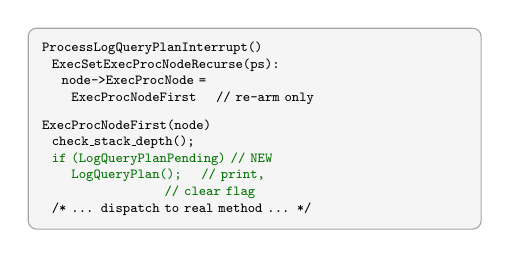
\begin{tikzpicture}
\node[draw=black!35, rounded corners=3pt, fill=black!4, align=left,
      font=\ttfamily\tiny, inner sep=5pt, text width=5.4cm]
{ProcessLogQueryPlanInterrupt()\\
~~ExecSetExecProcNodeRecurse(ps):\\
~~~~node->ExecProcNode =\\
~~~~~~ExecProcNodeFirst~~~~// re-arm only\\[4pt]
ExecProcNodeFirst(node)\\
~~check\_stack\_depth();\\
~~\textcolor{green!45!black}{if (LogQueryPlanPending)~// NEW}\\
~~~~~~\textcolor{green!45!black}{LogQueryPlan();~~~~// print,}\\
~~~~~~\textcolor{green!45!black}{~~~~~~~~~~~~~~~~~~~// clear flag}\\
~~/* ... dispatch to real method ... */};
\end{tikzpicture}

\vspace{1mm}
{\tiny Hop 2 swaps a function pointer --- \textbf{no EXPLAIN} runs here.
The printing happens later, inside the wrapper, at node entry.}
\end{column}

% ---- Right: coverage over the whole plan tree ----
\begin{column}{0.44\textwidth}
\centering
{\small\textbf{Every node re-armed $\Rightarrow$ prints once}}
\vspace{2mm}

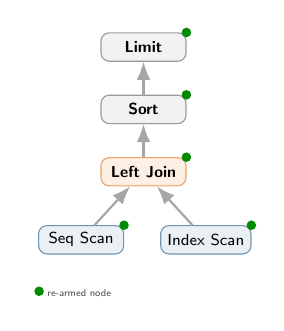
\begin{tikzpicture}[scale=0.72, every node/.append style={transform shape},
  op/.style={draw=black!40, rounded corners=3pt, fill=black!5,
             minimum height=0.5cm, minimum width=1.5cm,
             align=center, font=\sffamily\footnotesize},
  joinnode/.style={draw=pgorange!70, rounded corners=3pt, fill=pgorange!12,
             minimum height=0.5cm, minimum width=1.5cm,
             align=center, font=\sffamily\footnotesize},
  tbl/.style={draw=pgblue!70, rounded corners=3pt, fill=pgblue!10,
             minimum height=0.5cm, minimum width=1.5cm,
             align=center, font=\sffamily\footnotesize},
  edge/.style={thick, -Latex, gray!70},
]
\node[op]       (limit) at (0,  0.2)  {\textbf{Limit}};
\node[op]       (sort)  at (0, -0.9)  {\textbf{Sort}};
\node[joinnode] (lj)    at (0, -2.0)  {\textbf{Left Join}};
\node[tbl]      (seq)   at (-1.1, -3.2) {Seq Scan};
\node[tbl]      (idx)   at (1.1, -3.2)  {Index Scan};

\draw[edge] (seq)  -- (lj);
\draw[edge] (idx)  -- (lj);
\draw[edge] (lj)   -- (sort);
\draw[edge] (sort) -- (limit);

% Green badge = ExecProcNode re-armed to ExecProcNodeFirst.
\foreach \nd in {limit, sort, lj, seq, idx}
  \fill[green!55!black] (\nd.north east) circle (2.4pt);

\node[font=\sffamily\tiny, text=black!70, align=left, anchor=north west]
  at (-2.05, -3.9)
  {\tikz\fill[green!55!black] (0,0) circle (2.4pt);~re-armed node};
\end{tikzpicture}

\end{column}
\end{columns}

\vspace{2mm}
{\footnotesize \texttt{ExecSetExecProcNodeRecurse} follows
\texttt{lefttree}, \texttt{righttree}, \texttt{subPlan}, plus
Append / MergeAppend / BitmapAnd|Or / SubqueryScan / CteScan / CustomScan
--- so whichever node the executor enters next prints the plan, then
clears the flag. (A \texttt{WrapNodesInProgress} guard blocks re-entrant
requests.)}
\end{frame}

% ---------------------------------------------------------------------
% SLIDE 3 -- how the EXPLAIN string is built.
%
% LogQueryPlan() (explain_running.c) does everything in a private,
% throwaway memory context, so no allocation leaks into the running
% query's per-query context.  NewExplainState() enables only "costs"
% (analyze stays false), so the signalled EXPLAIN is a plain cost
% EXPLAIN of the ALREADY-BUILT PlanState tree: ExplainStringAssemble ->
% ExplainPrintPlan -> ExplainNode() recurse, reading each node's fields.
% It never calls ExecProcNode, i.e. it never advances the query.
% ---------------------------------------------------------------------
\begin{frame}\frametitle{How the EXPLAIN is built}
\vspace{-1mm}
\begin{columns}[T]

% ---- Left: the LogQueryPlan() sequence, inside a throwaway context ----
\begin{column}{0.54\textwidth}
\centering
{\small\textbf{A string, built in a throwaway context}}
\vspace{2mm}

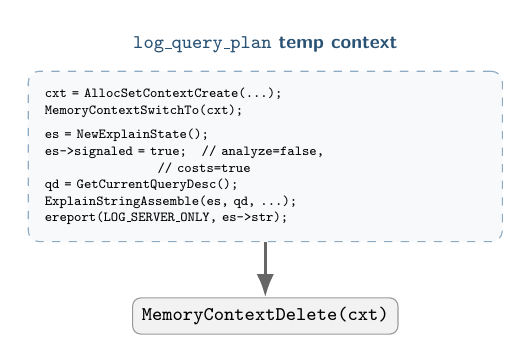
\begin{tikzpicture}
\node[draw=pgblue!55, dashed, rounded corners=4pt, fill=pgblue!4,
      align=left, font=\ttfamily\tiny, inner sep=6pt, text width=5.6cm] (ctx)
{cxt = AllocSetContextCreate(...);\\
MemoryContextSwitchTo(cxt);\\[3pt]
es = NewExplainState();\\
es->signaled = true;~~~// analyze=false,\\
~~~~~~~~~~~~~~~~~~~~~~~// costs=true\\
qd = GetCurrentQueryDesc();\\
\textbf{ExplainStringAssemble}(es, qd, ...);\\
ereport(LOG\_SERVER\_ONLY, es->str);};
\node[font=\sffamily\scriptsize\bfseries, text=pgblue!80!black,
      above=1mm of ctx.north] {\texttt{log\_query\_plan} temp context};
\node[draw=black!40, rounded corners=3pt, fill=black!5,
      font=\sffamily\scriptsize, below=7mm of ctx] (del)
  {\texttt{MemoryContextDelete(cxt)}};
\draw[very thick, -Latex, black!60] (ctx) -- (del);
\end{tikzpicture}

\vspace{1mm}
{\tiny Every EXPLAIN allocation lives in \texttt{cxt} and dies with it ---
nothing leaks into the running query's per-query context.}
\end{column}

% ---- Right: it walks the already-built plan tree, read-only ----
\begin{column}{0.44\textwidth}
\centering
{\small\textbf{It walks the tree that already exists}}
\vspace{2mm}

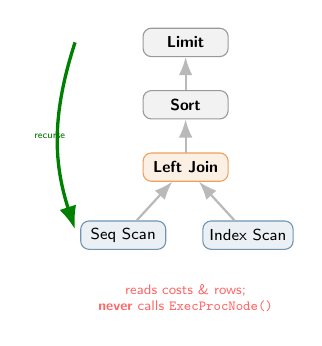
\begin{tikzpicture}[scale=0.72, every node/.append style={transform shape},
  op/.style={draw=black!40, rounded corners=3pt, fill=black!5,
             minimum height=0.5cm, minimum width=1.5cm,
             align=center, font=\sffamily\footnotesize},
  joinnode/.style={draw=pgorange!70, rounded corners=3pt, fill=pgorange!12,
             minimum height=0.5cm, minimum width=1.5cm,
             align=center, font=\sffamily\footnotesize},
  tbl/.style={draw=pgblue!70, rounded corners=3pt, fill=pgblue!10,
             minimum height=0.5cm, minimum width=1.5cm,
             align=center, font=\sffamily\footnotesize},
  edge/.style={thick, -Latex, gray!55},
]
\node[op]       (limit) at (0,  0.2)  {\textbf{Limit}};
\node[op]       (sort)  at (0, -0.9)  {\textbf{Sort}};
\node[joinnode] (lj)    at (0, -2.0)  {\textbf{Left Join}};
\node[tbl]      (s1)    at (-1.1, -3.2) {Seq Scan};
\node[tbl]      (s2)    at (1.1, -3.2)  {Index Scan};
\draw[edge] (s1)  -- (lj);
\draw[edge] (s2)  -- (lj);
\draw[edge] (lj)  -- (sort);
\draw[edge] (sort) -- (limit);

% Downward "recurse" arrow beside the tree (visual only).
\draw[very thick, -Latex, green!50!black] (-1.95, 0.2)
  to[bend right=18] (-1.95, -3.1);
\node[font=\sffamily\tiny, text=green!45!black, anchor=east] at (-2.0, -1.45)
  {recurse};
\node[font=\sffamily\scriptsize, text=red!60, align=center, anchor=north]
  at (0, -3.95) {reads costs \& rows;\\ \textbf{never} calls \texttt{ExecProcNode()}};
\end{tikzpicture}
\end{column}

\end{columns}

\vspace{1mm}
{\footnotesize No tuples pulled $\cdot$ private context $\cdot$
\texttt{analyze=false} $\Rightarrow$ a plain cost \texttt{EXPLAIN} of the
\emph{live} plan tree, assembled into one string and logged.}
\end{frame}

% ---------------------------------------------------------------------
% SLIDE 4 -- the one place EXPLAIN would touch executor state.
%
% ExplainNode() normally calls InstrEndLoop() to finalise the loop
% counters -- a MUTATION -- because at EXPLAIN ANALYZE time ExecutorEnd
% hasn't run yet.  For a signalled EXPLAIN of a RUNNING query that would
% corrupt the instrumentation the query is still updating, so the call
% is gated behind !es->signaled (explain.c:1878).  Combined with
% analyze=false, the assembler never writes to executor-owned state.
% ---------------------------------------------------------------------
\begin{frame}\frametitle{\ldots and why it can't touch the state}
\vspace{-1mm}
\begin{center}
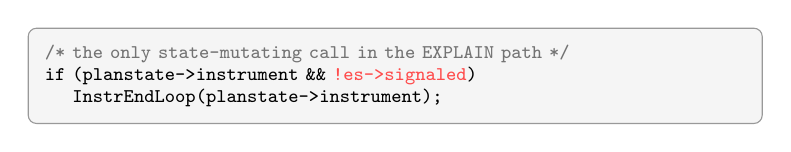
\begin{tikzpicture}
\node[draw=black!40, rounded corners=3pt, fill=black!4, align=left,
      font=\ttfamily\scriptsize, inner sep=6pt, text width=8.9cm]
{\textcolor{black!55}{/* the only state-mutating call in the EXPLAIN path */}\\
if (planstate->instrument \&\& \textcolor{red!70}{!es->signaled})\\
~~~~InstrEndLoop(planstate->instrument);};
\end{tikzpicture}
\end{center}

\vspace{1mm}
\begin{columns}[T]

\begin{column}{0.48\textwidth}
\centering
{\small\textbf{Normal \texttt{EXPLAIN ANALYZE}}}\\[1.5mm]
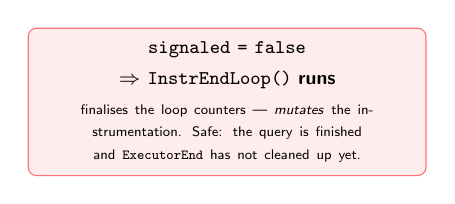
\begin{tikzpicture}
\node[draw=red!55, rounded corners=3pt, fill=red!7, align=center,
      font=\sffamily\scriptsize, inner sep=5pt, text width=4.7cm]
{\texttt{signaled = false}\\[3pt]
$\Rightarrow$ \texttt{InstrEndLoop()} \textbf{runs}\\[3pt]
{\tiny finalises the loop counters --- \emph{mutates} the
instrumentation. Safe: the query is finished and \texttt{ExecutorEnd}
has not cleaned up yet.}};
\end{tikzpicture}
\end{column}

\begin{column}{0.48\textwidth}
\centering
{\small\textbf{\texttt{pg\_log\_query\_plan()}}}\\[1.5mm]
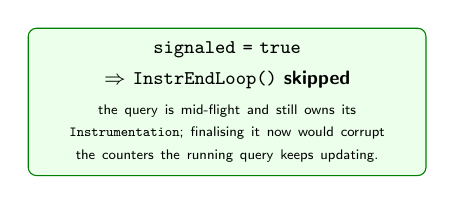
\begin{tikzpicture}
\node[draw=green!50!black, rounded corners=3pt, fill=green!8, align=center,
      font=\sffamily\scriptsize, inner sep=5pt, text width=4.7cm]
{\texttt{signaled = true}\\[3pt]
$\Rightarrow$ \texttt{InstrEndLoop()} \textbf{skipped}\\[3pt]
{\tiny the query is mid-flight and still owns its
\texttt{Instrumentation}; finalising it now would corrupt the counters
the running query keeps updating.}};
\end{tikzpicture}
\end{column}

\end{columns}

\vspace{2mm}
{\footnotesize With \texttt{signaled} \emph{and} \texttt{analyze=false}
(\texttt{NewExplainState} turns on only \texttt{costs}), the assembler
never writes to executor-owned state --- it only \emph{reads} the existing
\texttt{PlanState} tree.\hfill{\itshape explain.c:1878}}
\end{frame}

% ---------------------------------------------------------------------
% SLIDE 5 -- capstone: the full safety argument in one picture.
%
% The signal itself does almost nothing; three independent properties
% make the deferred print safe:
%   1. Safe point   -- printed at node entry (ExecProcNodeFirst), not at
%      an arbitrary interrupt.
%   2. Read-only    -- walks the already-built PlanState tree in a
%      private memory context; never calls ExecProcNode.
%   3. Gated write  -- InstrEndLoop (the one mutating call) skipped under
%      signaled; analyze=false so no live counters are read.
% The residual line keeps the reviewer honest: not eliminated, only made
% safe -- latency for a backend stuck inside one node, and the extension
% explain_per_plan_hook still fires on the signalled path.
% ---------------------------------------------------------------------
\begin{frame}\frametitle{Why the print is safe: three guarantees}
\vspace{-1mm}
\begin{center}
{\small The signal only \emph{arms} the print; three independent
properties make the print itself safe.}
\end{center}
\vspace{3mm}

\begin{center}
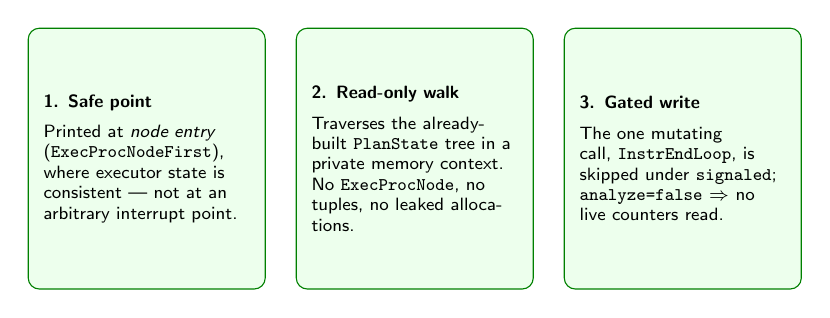
\begin{tikzpicture}[scale=0.92, every node/.append style={transform shape},
  pillar/.style={draw=green!50!black, rounded corners=4pt, fill=green!7,
    align=left, font=\sffamily\scriptsize, inner sep=6pt,
    text width=2.85cm, minimum height=3.6cm, anchor=north},
]
\node[pillar] (p1) at (-3.7, 1.8) {%
  \textbf{1. Safe point}\\[4pt]
  Printed at \emph{node entry}
  (\texttt{ExecProcNodeFirst}), where executor state is consistent ---
  not at an arbitrary interrupt point.};
\node[pillar] (p2) at (0, 1.8) {%
  \textbf{2. Read-only walk}\\[4pt]
  Traverses the already-built \texttt{PlanState} tree in a private
  memory context. No \texttt{ExecProcNode}, no tuples, no leaked
  allocations.};
\node[pillar] (p3) at (3.7, 1.8) {%
  \textbf{3. Gated write}\\[4pt]
  The one mutating call, \texttt{InstrEndLoop}, is skipped under
  \texttt{signaled}; \texttt{analyze=false} $\Rightarrow$ no live
  counters read.};
\end{tikzpicture}
\end{center}

\vspace{2mm}
{\footnotesize\itshape\color{black!60} Residual, not eliminated: a backend
stuck \emph{inside} one long node logs only when it next advances; and an
extension's \texttt{explain\_per\_plan\_hook} still fires on the signalled
path.}
\end{frame}

\end{document}
